\section{The Agent}

\subsection{Create Customer Profile}
\textbf{Pre-conditions}: The Agent must be logged into the system.

\textbf{Post-conditions}: Customer successfully created a profile.

\textbf{Purpose}: The agent wants to be able to add customers to the system
in order to buy tickets for them.

\textbf{Description}: The user fills in the form with the customer details
and presses the save button. Once all the details are saved, the system
notifies the user that all the changes have been saved.

\subsection{Buy tickets}
\textbf{Pre-conditions}: An agent must be logged in into the system and
at least one event and one show exist on the system, as well as one customer that is managed by
the agent.

\textbf{Post-conditions}: Tickets have been bought by an agent on behalf of
a customer at the right price with the agent's commission.

\textbf{Purpose}: The agent wants to be able to sell tickets for his customers
in order to gain money and commission, and to have the tickets reserved for the
right person

\textbf{Description}: The user selects the customer he wants to buy tickets for and
presses OK, the system then prompts the user to select the event they want to buy
tickets for. The user selects the event and then presses OK, and then a list of the
available shows appears with the number of seats available for the agent to sell
for this show. The agent then selects the show and presses OK. The user is then
prompted to choose the number of tickets that he wants to buy, and the user selects
the number and presses OK. The system then displays the seats that are available
for the agent to reserve. The agent selects the seats to be reserved according to
the number of tickets that they are buying and then select OK. The total price
for the tickets then appears in the system, explaining which values are for
the tickets and which are for the agent's commission, then the user presses
the Pay button to complete the purchase.

\subsection{Update Customer Profiles}
\textbf{Pre-conditions}: An agent is logged into the system and at least
one customer profile managed by this manager exists in the system.

\textbf{Post-conditions}: A profile managed by an agent is updated

\textbf{Purpose}: An agent wants to make changes to the information
held in the profile of a customer that they manage (name, address,
payment information, etc.)

\textbf{Description}: The system provides to the user a list of the
users that they manage and the user selects the user to which
they want to change the information. A form then appears holding the
current information of the customer. The user changes the information
necessary and when they are happy with the changes they press the save
button. When all the changes have been saved, the system notifies
the user that the changes have been successfully been applied.

\subsection{View Sold Tickets}
\textbf{Pre-conditions}: An agent is logged into the system.

\textbf{Post-conditions}: A list with the tickets sold and the total number
of tickets that the agent has sold either for a show or for a range of dates
are displayed to the user.

\textbf{Purpose}: An agent wants to see how many tickets they have sold in the
platform, either for a particular show or for all shows in a date range.

\textbf{Description}: The system ask the user if they want to see the tickets that
they have sold for a show or for a specific date range. The user selects one of the two
options. If they have selected a show, the system will display a list of events, from
which the user must choose an event, then a list of shows for that event. The user then
selects the show and the list of sold tickets and the total number of tickets is shown
to the user. In case the user wants to see the tickets that they have sold for a date
range, the user selects the begin date of the search and then the end date of the
search and the system will then display all the tickets sold and the total number of
tickets.

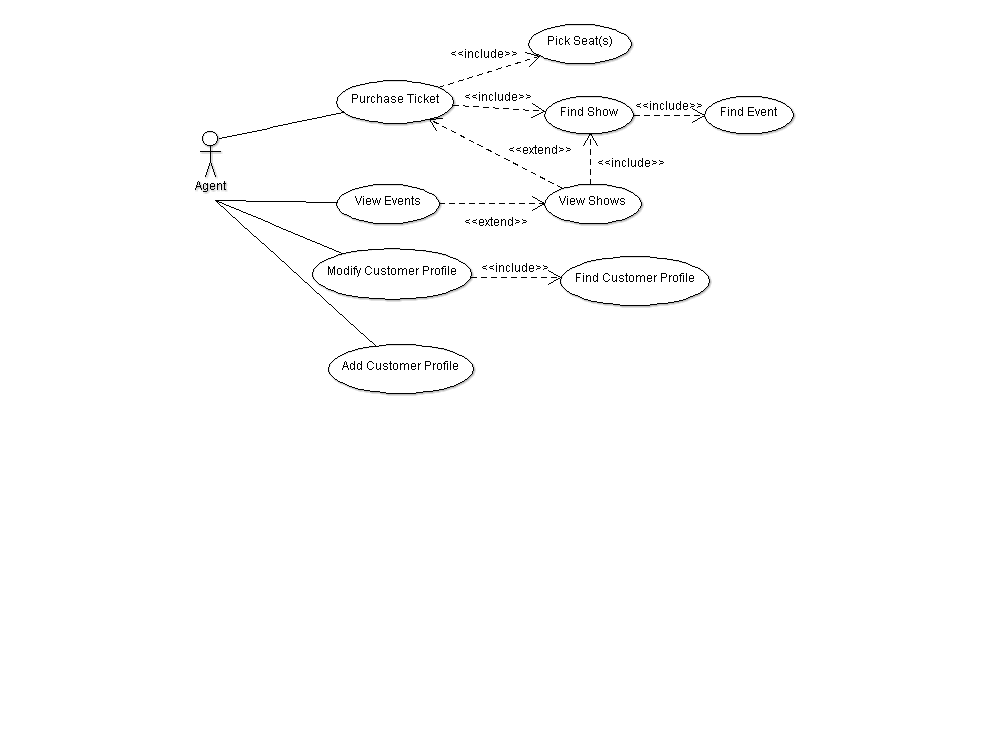
\includegraphics[width=\linewidth]{AgentUsecaseDiagram}
